\documentclass[11pt, a4paper, landscape]{article}
\usepackage[english,userlastpage,triangle,utf-8]{NeyDreuwSlides_Oct08}
\usepackage{algorithm}
\usepackage{algpseudocode}
\usepackage{tikz}
\usepackage{pifont}
\usepackage{wasysym}
\usepackage{amssymb}
\usepackage{pdfpages}
\usepackage{color}

\renewcommand*{\title}{ASR Lab Results}                               % main title of the work (used for \TitlePage)
\renewcommand*{\titleshort}{ASR Lab Results}                    % short title (used for \lfoot)
\renewcommand*{\occasion}{Presentation} % (used for \TitlePage)
\renewcommand*{\occasionshort}{~}  % short occasion title (used for \rfoot)
\renewcommand*{\date}{\today}
\renewcommand*{\author}{Ilya Sklyar, Konstantin Kromberg, Miguel Gra\c{c}a}                                     % all the authors of the work, can be long (used for \TitlePage)
\renewcommand*{\authorshort}{Sklyar, Kromberg, Gra\c{c}a~~}                                        % all the authors of the work, should be short (used for \lfoot)
\renewcommand*{\email}{~}             % all email address(es) of the authors (used for \TitlePage)
\renewcommand*{\mainauthor}{Ilya Sklyar, Konstantin Kromberg, Miguel Gra\c{c}a}                                 % the author(s) who presented the work (used for \FinalPage)
\renewcommand*{\mainauthoremail}{\email}                                  % presenter mail address(es) (used for \FinalPage)
\renewcommand*{\www}{~}            % web address (used for \TitlePage _and_ \FinalPage)
\newcommand*{\keywords}{Title of Presentation, etc.}      % keywords for pdf summary
\renewcommand{\arraystretch}{1.2}

% will be set into the PDF document summary
\hypersetup{
  pdftitle={\title}, 
  pdfsubject={\occasion},  
  pdfauthor={\author}, 
  pdfkeywords={\keywords}
}

%%%%%%%%%%%%%%%%%%%%%%%%%%%%%%%%%%%%%%%%%%%%%%%%%%%%%%%%%%%%%%%%%%%%%%%%%%%%%%%%
\usepackage[insection]{minitoc}
\renewcommand{\stifont}{\normalsize\bf} 
\renewcommand{\stcfont}{\normalsize\bf}
\renewcommand{\stcSSfont}{\normalsize\bf}

\begin{document}

%%%%%%%%%%%%%%%%%%%%%%%%%%%%%%%%%%%%%%%%%%%%%%%%%
\TitlePage

%%%%%%%%%%%%%%%%%%%%%%%%%%%%%%%%%%%%%%%%%%%%%%%%%
\NewPage\headline{Overview}
\vfill
\begin{itemize}
  \item Gaussian Mixture Model (GMM) tuning
  \begin{itemize}
    \item Expectation-Maximization (EM) parameters
    \item Alignment parameters
    \item Search results
  \end{itemize}
  \item Neural Network (NN) tuning
  \begin{itemize}
    \item Training parameters
    \item Search results
  \end{itemize}
  \item Tuned results
\end{itemize}
\vfill

%%%%%%%%%%%%%%%%%%%%%%%%%%%%%%%%%%%%%%%%%%%%%%%%%
\NewPage\headline{GMM tuning: EM parameters}
\vfill
Basic setup:
\begin{itemize}
%  \item Lexicon consists of 106 states
  \item 0-1-2 6 state HMM topology on phoneme-level $\Rightarrow$ 106 total states
  \item Exact computation of the linear segmentation
  \item Maximum approximation for GMMs
  \item 6 EM steps
  \item 4 density splits
\end{itemize} 
\vspace{20pt}
Tunable properties:
\begin{itemize}
  \item Minimum observations per density
  \item Pooling type
\end{itemize}
\vspace{20pt}
Tuning is based on the likelihood of the training data
\vfill

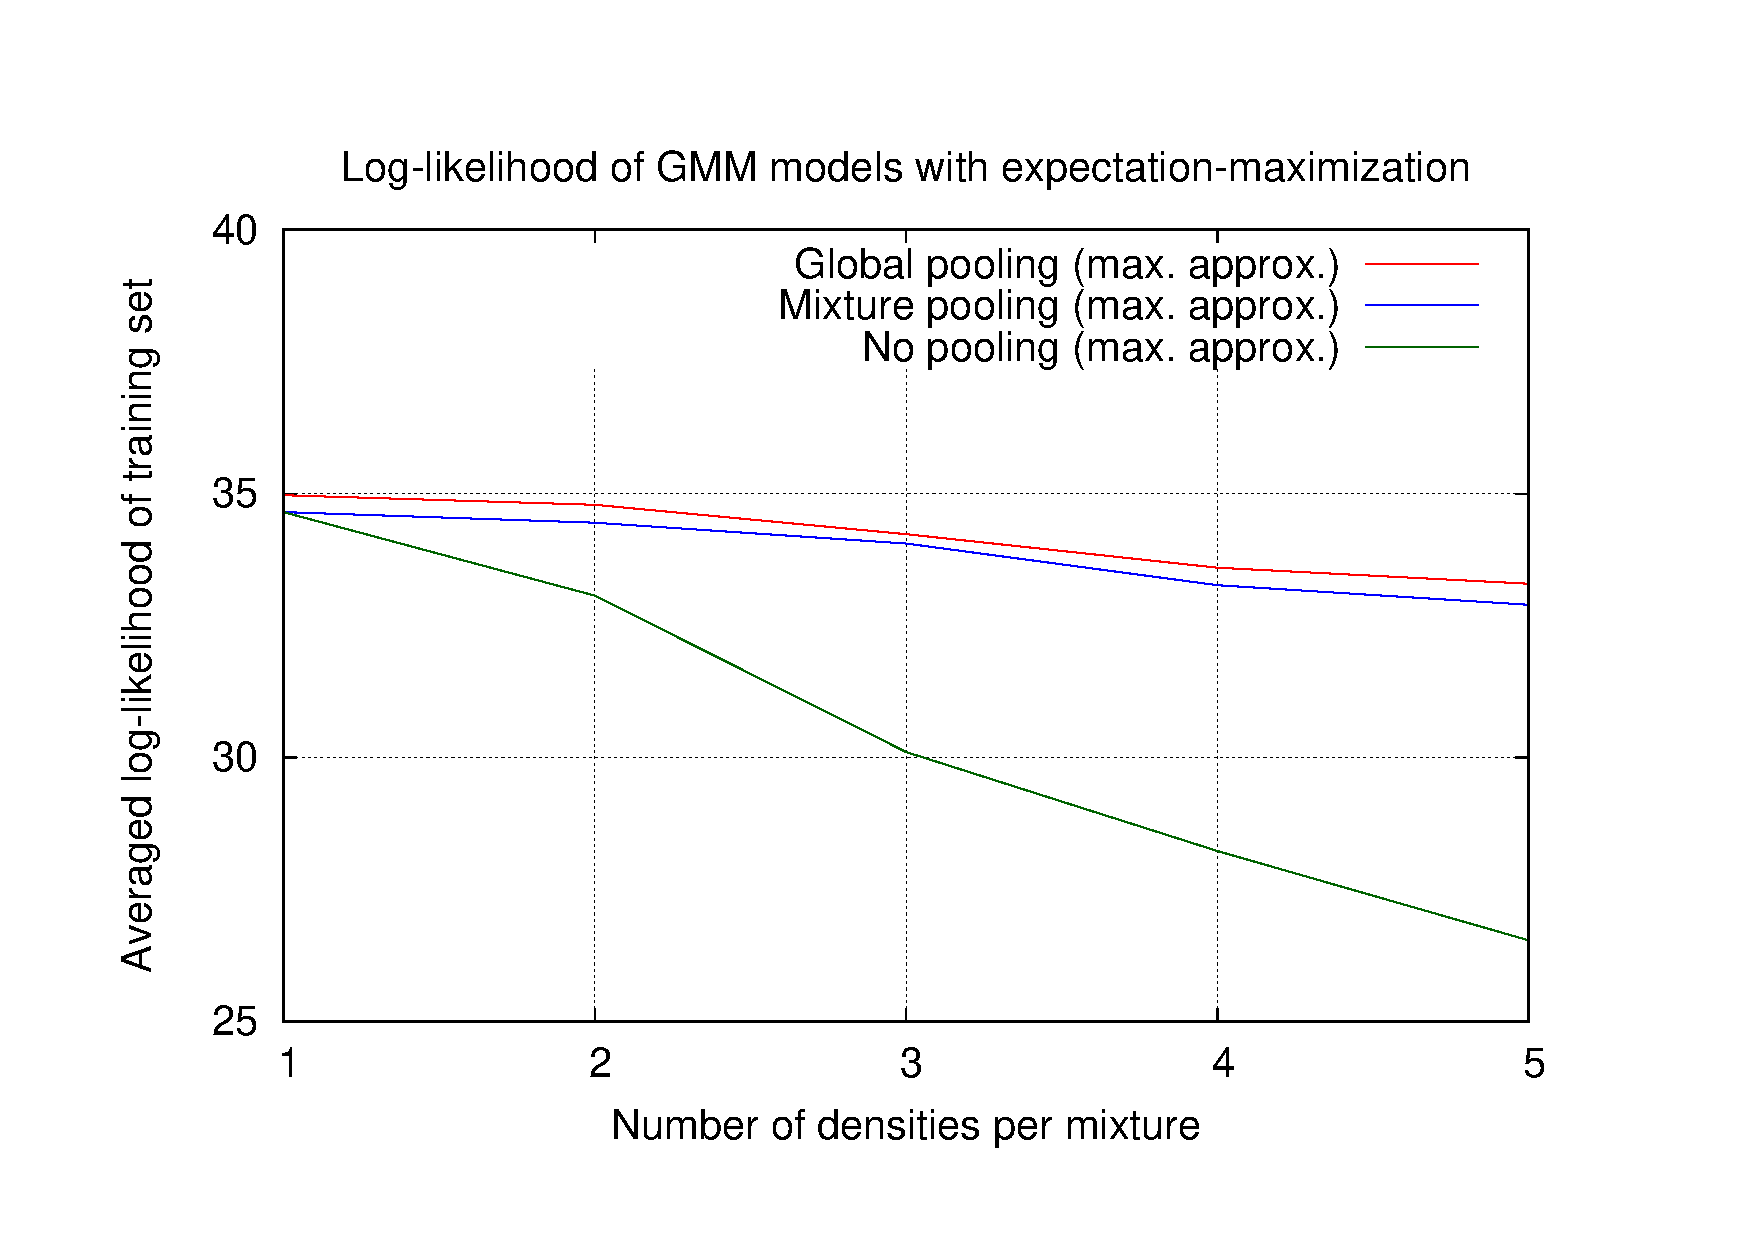
\includepdf[pages=-]{plots/am_score_afterSplit.pdf} 

%%%%%%%%%%%%%%%%%%%%%%%%%%%%%%%%%%%%%%%%%%%%%%%%%%%
\NewPage\headline{GMM tuning: EM parameters}
\vfill
Pooling:
\begin{itemize}
	\item No pooling results in better model fitting than using pooling 
	\item Global and mixture-level pooling perform similarly 
	\item We infer, that due to the size of data set, pooling isn't necessary
\end{itemize}
\vspace{20pt}
Splitting criterion:
\begin{itemize}
	\item Minimum number of observations per density has a small influence
	\item Sufficient data points per density in a mixture due to:
	\begin{itemize}
		\item At most $5$ densities per mixture
		\item Each density has, in average, $7$K data points.
	\end{itemize}
\end{itemize}
\vfill

%%%%%%%%%%%%%%%%%%%%%%%%%%%%%%%%%%%%%%%%%%%%%%%%
\NewPage\headline{GMM tuning: Alignment parameters}
\vfill
Setup:
\begin{itemize}
  \item Viterbi approximation
  \item Pruning threshold of 200 (tuned on previous assignment) 
\end{itemize}
\vspace{20pt}
Tunable parameters (optimized on the best performing EM setup):
\begin{itemize}
	\item Time distortion penalty (TDP) values:
    \begin{itemize}
      \item Forward transitions do not have costs (to enforce monotonicity)
      \item Skip and loop transitions have differing costs
      \item Due to high number of states per word, skips should cost more
    \end{itemize}
\end{itemize}
\vfill

%%%%%%%%%%%%%%%%%%%%%%%%%%%%%%%%%%%%%%%%%%%%%%%%
\NewPage\headline{Alignment results}
\vfill
\begin{itemize}
  \item Evaluation on acoustic model (AM) score and silence ratio in alignments
  \item TDP format (Loop-Forward-Skip) 
\end{itemize}

\begin{center}
\begin{tabular}{| l |  c | c |} \toprule
  TDP        & AM score           & Silence [\%]      \\ \midrule
  1-0-10     & \color{red}{22.68} & \color{red}{43.48}\\
  2-0-20     & 22.73              & 53.20             \\
  3-0-30     & 23.05              & 59.60             \\ \midrule
  10-0-10    & 23.98              & 75.61             \\
  20-0-20    & 24.31              & 80.35             \\
  30-0-30    & 24.37              & 80.35             \\ \bottomrule
\end{tabular}
\end{center}
\vspace{10pt}
\begin{itemize}
	\item Cheaper loop transitions results in alignments with less silence
	\item First 3 systems have similar AM scores, but differing silence ratios
  \begin{itemize}
    \item Find best performing system based on word error rate in search
  \end{itemize}
\end{itemize}
\vfill


%%%%%%%%%%%%%%%%%%%%%%%%%%%%%%%%%%%%%%%%%%%%%%%%
\NewPage\headline{Search results}
\vfill
Recognition setup:
\begin{itemize}
	\item Pruning threshold of 200
	\item Tuning evaluated on the whole test corpus for each GMM model
\end{itemize}
\vspace{20pt}
Tuned parameters to minimize word error rate (WER):
\begin{itemize}	
	\item Word penalty (in range 60 to 120)
\end{itemize}

%\begin{center}
%	\begin{tabular}{| l | c |} \toprule
%		WP / TDP       &    WER [\%]     \\ \midrule
%		100 / 1-0-10   &    7.29         \\
%		80 ~~/ 2-0-20   &    5.19         \\
%		80 ~~/ 3-0-30   &\color{red}{4.70}\\ \midrule
%		80 ~/ 10-0-10  &    10.09        \\
%		60 ~/ 20-0-20  &    13.35        \\
%		60 ~/ 30-0-30  &    13.69        \\ \bottomrule		
%	\end{tabular}
%\end{center}

\begin{center}
	\begin{tabular}{| l | l | c |} \toprule
		WP  &  TDP      &    WER [\%]     \\ \midrule
		100 &  1-0-10   &    7.29         \\
		80  &  2-0-20   &    5.19         \\
		80  &  3-0-30   &\color{red}{4.70}\\ \midrule
		80  &  10-0-10  &    10.09        \\
		60  &  20-0-20  &    13.35        \\
		60  &  30-0-30  &    13.69        \\ \bottomrule		
	\end{tabular}
\end{center}
%
%Results for whole corpus 80/2-0-20:
%\begin{itemize}
%	\item WER: 4.63\% SER: 12.03\%  RTF: 0.37
%\end{itemize}
\vfill

%%%%%%%%%%%%%%%%%%%%%%%%%%%%%%%%%%%%%%%%%%%%%%%%
\NewPage\headline{Neural Network Tuning}
Basic setup:
\begin{itemize}
  \item Output layer 106 (number of states in the alignment)
  \item Batch size 32 
  \item Tanh nonlinearity
  \item Adadelta updater
  \item Cross-validation (CV) size 10\%
  \item Best alignment from GMM Training
\end{itemize}
\vspace{20pt}
Tunable parameters:
\begin{itemize}
	\item Number of context frames (CF)
	\item Number of layers
	\item Number of nodes on each layer
	\item Number of epochs
	\item Search parameters: TDP and WP
\end{itemize}

%%%%%%%%%%%%%%%%%%%%%%%%%%%%%%%%%%%%%%%%%%%%%%%%
\NewPage\headline{Search Results}
\vfill
\begin{center}
\begin{table}[]
	\centering
\textbf{
	\begin{tabular}{|c|c|c|c|c|c|c|c|} \toprule
		\begin{tabular}[c]{@{}l@{}}Layers\end{tabular} & \begin{tabular}[c]{@{}l@{}}Nodes\end{tabular} & \begin{tabular}[c]{@{}l@{}}CF\end{tabular} & Epoch & TDP & WP  & FER (CV) {[}\%{]} & WER {[}\%{]} \\ \midrule
1  &  150          &  2  &  15  &  4-0-30  &  105  &  20.91  &  \color{red}{25.34}  \\
2  &  100-100      &  2  &  12  &  3-0-30  &  90  &  22.3   &  33.01  \\
7  &  100 each     &  2  &  10  &  2-0-20  &  80  &  22.7   &  36.33  \\
1  &  100          &  0  &  19  &  5-0-20  &  70  &  25.44  &  40.14  \\
3  &  500-300-100  &  2  &  18  &  5-0-0   &  70  &  18.65  &  41.3   \\
		 \bottomrule
	\end{tabular}
}
\end{table}
\end{center}

Conclusion:
\begin{itemize}
	\item Frame error rate (FER) does not correlate with WER
	\item Shallow networks perform better than deeper ones
	\item Results are still much worse than GMM
\end{itemize}

%%%%%%%%%%%%%%%%%%%%%%%%%%%%%%%%%%%%%%%%%%%%%%%%%
\NewPage\headline{Tuned results}
\vfill
\begin{itemize}
  \item CPU: Intel(R) Xeon(R) E3-1230 v3 @ 3.30GHz with SSE2 registers
  \item Results for our best performing systems
  \item Speed results in real-time factor (RTF) or in elapsed time
\end{itemize}

\begin{table}[]
\centering
\textbf{
\begin{tabular}{| l | c | c | c | c | c | } \toprule
Search & WER [\%] & SER [\%] & RTF 1 thread & RTF 4 threads  \\ \midrule
GMM    & 4.7      & 12.34    & 0.21         & 0.08           \\
NN     & 25.34    &          & 0.31         & 0.31           \\ \bottomrule
\end{tabular}
}
\end{table}

\begin{table}[]
\centering
\textbf{
\begin{tabular}{| l | c | c | c |} \toprule
Training & Time[s]  1 thread & Time[s] 4 threads  \\ \midrule
GMM      &  668.1            &  668.1             \\
NN       &  4717.1           &  3967.4            \\ \bottomrule
\end{tabular}
}
\end{table}

\begin{itemize}
  \item GMMs outperform NNs in both speed and error rates
\end{itemize}
\vfill

\FinalPage
\end{document}
